\documentclass[conference]{IEEEtran}
\IEEEoverridecommandlockouts
\usepackage{cite}
\usepackage{amsmath,amssymb,amsfonts}
\usepackage{graphicx}
\usepackage{textcomp}
\usepackage{xcolor}
\usepackage{booktabs}
\usepackage{dblfloatfix}
\usepackage{url}
\usepackage[hidelinks]{hyperref}
\setlength{\floatsep}{6pt plus 2pt minus 2pt}
\setlength{\textfloatsep}{8pt plus 2pt minus 2pt}
\setlength{\intextsep}{6pt plus 2pt minus 2pt}
\setlength{\abovecaptionskip}{4pt}
\setlength{\belowcaptionskip}{2pt}
\def\BibTeX{{\rm B\kern-.05em{\sc i\kern-.025em b}\kern-.08em
  T\kern-.1667em\lower.7ex\hbox{E}\kern-.125emX}}

\begin{document}

\title{A Lightweight Domain-Generalized and Uncertainty-Aware Framework for Reliable Cross-Dataset Diabetic Foot Ulcer Segmentation}

\author{
\IEEEauthorblockN{Nagesh Ragolu, Sali Soumith, Abhigna Rao Lingala,\\
Donepudi Harshita, R.\ Varshitha Sree, and Pandu Sowkuntla}
\IEEEauthorblockA{Department of Computer Science and Engineering,\\
SRM University-AP, Vijayawada, Andhra Pradesh, India\\
Corresponding author: Nagesh Ragolu (ragolunagesh@gmail.com)}
}

\maketitle

\begin{abstract}
Deep-learning segmentation models for diabetic foot ulcers (DFUs) often perform well on the dataset used for training but degrade when images are acquired under different clinical, colour, and illumination conditions. This paper presents MobileDFU-Net, a lightweight segmentation framework that combines a decoupled chromatic--structural stem with raw-RGB input, a tolerance-aware signed-distance boundary loss, and Monte Carlo (MC) Dropout inference that produces predictive entropy and mutual information. An audited data-reconciliation process identified only two independent lineage groups (AZH and WSEG/Mendeley) and established an approved source-only population of 927 training and 186 internal-validation records, with a native target cohort of 2,187 records reserved for cross-dataset evaluation. Three source-domain training runs (seeds 42, 1337, 2024) reached best internal-validation Dice scores of 0.8370, 0.8322, and 0.8326 (mean 0.8339 $\pm$ 0.0027). On the native target cohort the same checkpoints obtained macro Dice of 0.2485, 0.2365, and 0.2203, showing severe foreground under-segmentation. Increasing the segmentation positive-class weight from 2 to 4 raised native Dice only from 0.2365 to 0.2436 and sensitivity from 0.1933 to 0.2110, missing the predefined targets. Entropy- and mutual-information-based failure detection was anti-correlated with failure (AUROC 0.300 and 0.311 for Dice $<$ 0.1), i.e., the model was often confidently wrong. Removing the colour stem or the boundary signal also degraded native Dice (0.2398 and 0.2067). We report these negative findings explicitly and treat the domain gap, foreground suppression, and uncertainty reliability as open problems rather than solved ones.
\end{abstract}

\begin{IEEEkeywords}
diabetic foot ulcer, medical image segmentation, domain generalization, cross-dataset evaluation, boundary-aware learning, Monte Carlo dropout, uncertainty estimation, lightweight neural networks
\end{IEEEkeywords}

\section{Introduction}
\label{sec:intro}

Diabetic foot ulcers (DFUs) are a major complication of diabetes mellitus and require consistent wound assessment for monitoring and treatment planning. Automated segmentation of DFU regions from clinical photographs can support wound-area quantification and healing tracking. A well-documented limitation of deep segmentation models is that performance on a held-out split of the training dataset does not reliably predict performance on images from another clinical site, camera, or lighting setup \cite{Zhou2023DomainGeneralization}. The problem is acute in wound photography, where skin tone, ambient light, white balance, and acquisition protocol alter colour statistics without changing the underlying pathology \cite{Wang2024FUSeg,Cassidy2021DFUC2020}.

This paper is organized around reliable cross-dataset DFU segmentation. Uncertainty estimation and failure detection are secondary objectives that support reliability assessment; colour-robust feature learning and boundary-aware segmentation are supporting components rather than the primary claim. We use DFU-FuzzyLiteUNet \cite{Purwono2025DFUFuzzyLiteUNet} only as an example of how a complete DFU segmentation study can be organized: its fuzzy sigmoid, lite-transformer block, datasets, and reported scores belong to that work and are not part of MobileDFU-Net.

The contributions supported by completed, artifact-verified evidence are:
\begin{itemize}
\item An audited lineage-reconciliation process that reduced several candidate wound-image sources to two independent lineage groups and froze an approved source-only population (927 training, 186 internal-validation records) plus a native target cohort (2,187 records).
\item MobileDFU-Net, a 1,116,883-parameter encoder--decoder with a decoupled chromatic--structural stem, an inverted-residual encoder, a receptive-field-block bottleneck, a lightweight decoder, and an auxiliary boundary head.
\item A colour contract that preserves raw RGB in $[0,1]$ and confines ImageNet normalization to an internal chromatic branch, so source colour statistics are not baked into the data pipeline.
\item A tolerance-aware signed-distance boundary loss adapted from Kervadec \emph{et al.} \cite{Kervadec2019BoundaryLoss}, with $3\times3$ erosion, a Euclidean distance transform, $\tau=2$, and a distance cap of 20.
\item An MC Dropout inference path \cite{Gal2016DropoutBayesian,Houlsby2011BALD} with $T=15$ passes, horizontal-flip test-time augmentation (TTA), predictive entropy, and mutual information.
\item Three source-only training runs and a frozen native-target evaluation, including two negative ablations and one negative recovery intervention, reported without selective omission.
\end{itemize}

\begin{figure*}[!tb]
\centering
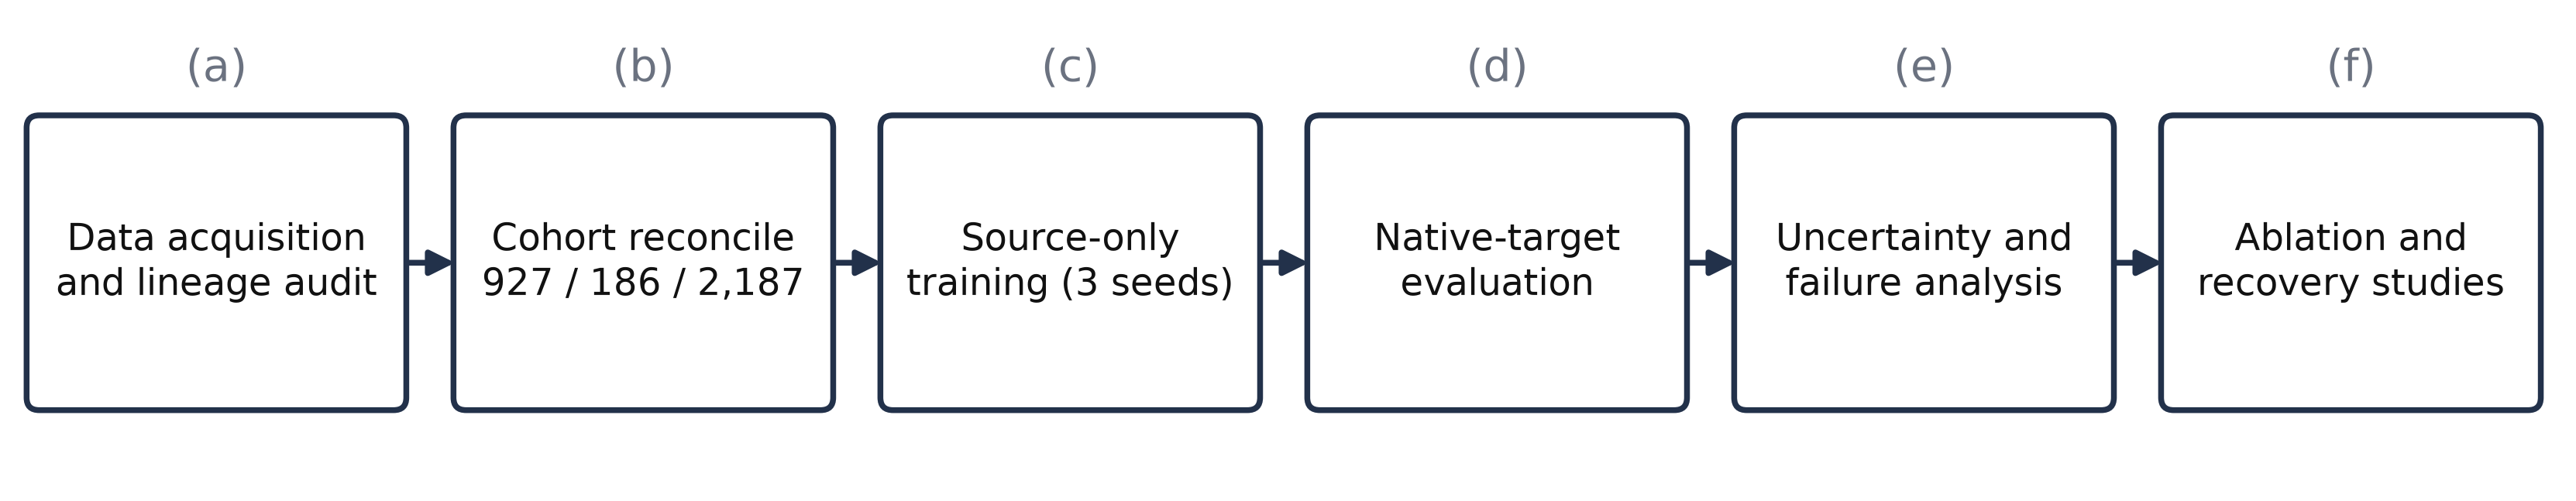
\includegraphics[width=\textwidth]{figures/fig1_workflow.png}
\caption{Research workflow: data acquisition and lineage audit, cohort reconciliation (927 training / 186 internal validation / 2,187 native target), source-only training with three seeds, native-target evaluation, uncertainty and failure analysis, and ablation/recovery studies.}
\label{fig:workflow}
\end{figure*}

\section{Related Work}
\label{sec:related}

\textbf{DFU and wound segmentation.} Convolutional encoder--decoders are widely used for wound and DFU segmentation \cite{Wang2015WoundSegmentation}. U-Net \cite{Ronneberger2015UNet} and its self-configuring variant nnU-Net \cite{Isensee2021nnUNet} remain strong general-purpose baselines. DFU-FuzzyLiteUNet \cite{Purwono2025DFUFuzzyLiteUNet} is a recent lightweight U-Net with a fuzzy sigmoid and a lite transformer block, evaluated on FUSeg 2021 and DFUC 2022. Reported within-dataset scores in this line of work are often high, whereas cross-dataset evaluation is less frequently reported; this motivates our emphasis on lineage auditing and a frozen target protocol.

\textbf{Domain generalization and adaptation.} Domain shift across sites, devices, and protocols is a recognized obstacle to deployment \cite{Zhou2023DomainGeneralization}. Medical-imaging surveys organize the field into feature normalization, adversarial alignment, reconstruction, and disentangled representation learning \cite{Guan2021DomainAdaptation}. Multi-source domain generalization has been approached with domain- and content-adaptive convolution \cite{Hu2023DCAConv}. Our contribution is deliberately narrower: a raw-RGB input contract and a structure-conditioned colour gate, not a new general framework.

\textbf{Boundary-aware losses.} Distance-transform boundary losses improve irregular or low-contrast boundaries \cite{Kervadec2019BoundaryLoss}. We adapt the signed-distance linear form and keep its tolerance band explicit.

\textbf{Uncertainty estimation.} MC Dropout approximates Bayesian inference without architectural change \cite{Gal2016DropoutBayesian}. Predictive entropy measures total uncertainty, while mutual information isolates the epistemic component via the BALD decomposition \cite{Houlsby2011BALD}. Calibration is a separate property and is not guaranteed by uncertainty estimation \cite{Guo2017Calibration}; aleatory and epistemic uncertainties must also be distinguished carefully \cite{Kendall2017Uncertainties}.

\textbf{Lightweight segmentation.} Inverted residual blocks \cite{Sandler2018MobileNetV2} and multi-scale receptive-field modules \cite{Liu2018RFBNet} reduce cost for resource-constrained deployment. MobileDFU-Net follows this design philosophy.

\section{Problem Formulation and Metrics}
\label{sec:problem}

Let $\mathcal{D}_S=\{(x_i,y_i)\}_{i=1}^{N_S}$ be a source dataset of DFU images $x_i\in\mathbb{R}^{3\times H\times W}$ and binary masks $y_i\in\{0,1\}^{1\times H\times W}$, and let $\mathcal{D}_T$ be a native target dataset from a distinct lineage with a different acquisition and colour distribution. A model $f$ trained on $\mathcal{D}_S$ generalizes across datasets if its performance on $\mathcal{D}_T$ approaches its performance on a held-out split of $\mathcal{D}_S$. We train and validate on $\mathcal{D}_S$ and evaluate once on the frozen $\mathcal{D}_T$.

For image $i$, with true positives TP$_i$, false positives FP$_i$, false negatives FN$_i$, and true negatives TN$_i$ at threshold $\tau$, the hard-threshold metrics are
\begin{equation}
\mathrm{Dice}_i=\frac{2\,\mathrm{TP}_i}{2\,\mathrm{TP}_i+\mathrm{FP}_i+\mathrm{FN}_i},
\label{eq:dice}
\end{equation}
\begin{equation}
\mathrm{IoU}_i=\frac{\mathrm{TP}_i}{\mathrm{TP}_i+\mathrm{FP}_i+\mathrm{FN}_i},\quad
\mathrm{Sens}_i=\frac{\mathrm{TP}_i}{\mathrm{TP}_i+\mathrm{FN}_i},
\label{eq:iou_sens}
\end{equation}
\begin{equation}
\mathrm{Spec}_i=\frac{\mathrm{TN}_i}{\mathrm{TN}_i+\mathrm{FP}_i}.
\label{eq:spec}
\end{equation}
Empty ground truth and empty prediction are scored as Dice $=$ IoU $=1$, following the evaluation implementation; undefined sensitivity or specificity for an empty reference is excluded from the corresponding macro average. Macro and micro Dice are
\begin{equation}
\mathrm{Dice}_{\mathrm{macro}}=\frac{1}{N}\sum_{i=1}^{N}\mathrm{Dice}_i,
\label{eq:macro}
\end{equation}
\begin{equation}
\mathrm{Dice}_{\mathrm{micro}}=\frac{2\sum_i \mathrm{TP}_i}{2\sum_i\mathrm{TP}_i+\sum_i\mathrm{FP}_i+\sum_i\mathrm{FN}_i}.
\label{eq:micro}
\end{equation}
The three-seed summary is the sample mean $\bar{m}$ and sample standard deviation $s$ of the three best internal-validation Dice values; it describes seed dispersion on one cohort and is neither a confidence interval nor a cross-validation result.

\section{Materials and Methods}
\label{sec:method}

\subsection{Dataset Reconciliation and Cohort Definition}

Candidate resources included the AZH wound dataset, a WSEG dataset, a Mendeley wound-image dataset, FUSeg 2021 \cite{Wang2024FUSeg}, and DFUC 2022. FUSeg required manual account verification, and the DFUC 2022 challenge required institutional authorization and a signed licence; DFUC 2022 was therefore not used experimentally, and the DFUC 2020 dataset paper \cite{Cassidy2021DFUC2020} is cited only for context. A lineage audit found that the downloaded archives reduce to two independent groups: AZH, and WSEG/Mendeley, which share lineage with each other; AZH additionally shares lineage with FUSeg. The evidence therefore does not support a claim of broad, multi-centre, independent external validation.

\begin{table}[!t]
\centering
\caption{Dataset cohorts and approved analysis populations}
\label{tab:cohorts}
\begin{tabular}{@{}lr@{}}
\toprule
Cohort & Records \\
\midrule
Source training, before exclusions & 945 \\
Internal validation, before exclusions & 191 \\
Native target cohort & 2,187 \\
\midrule
Approved source-training exclusions & 18 \\
Approved internal-validation exclusions & 5 \\
\midrule
Approved source-training population & 927 \\
Approved internal-validation population & 186 \\
\bottomrule
\end{tabular}
\end{table}

The manifest contained 193 internal-validation rows. Deduplication of primary contents left 192 unique primary rows; one of these (\texttt{val\_img\_0233}) is flagged \texttt{is\_diagnostic=True} with task \texttt{diagnostic\_multiclass} and is not an eligible binary primary, leaving 191 eligible primaries, exactly the pre-exclusion count in Table~\ref{tab:cohorts}. Five label-uncertain records were then excluded, giving 186. Source training started from 945 records, 18 were excluded, giving 927. The 2,187 native-target records were excluded from every training run.

\subsection{Preprocessing Contract}

Images are RGB float32 in $[0,1]$ with layout $[3,H,W]$ and no dataset-level ImageNet normalization. Masks are float32 $[1,H,W]$ with values $\{0,1\}$. Images and masks are letterbox-resized to $512\times512$ with aspect-ratio preservation and zero padding, using bilinear interpolation for images and nearest-neighbour for masks. The contract is identical for source training, internal validation, and the native target. Augmentation is applied only to source training; geometric transforms are shared by image and mask, boundary fields are recomputed after geometric augmentation, and randomness is seeded from the training seed, record identifier, and epoch.

\subsection{MobileDFU-Net Architecture}

MobileDFU-Net (Fig.~\ref{fig:architecture}) comprises (i) a decoupled chromatic--structural stem (DCS-Stem) producing 24 channels at $512^2$; (ii) an inverted-residual encoder with widths $(24,32,64,128)$, block counts $(2,3,4,3)$, and stride 2 per stage, producing stage features S1--S4 at $256^2$, $128^2$, $64^2$, and $32^2$; (iii) a receptive-field-block bottleneck \cite{Liu2018RFBNet} with four parallel dilated branches and 160 channels at $32^2$; (iv) a decoder with four upsampling stages Up4--Up1, whose output widths are $(96,48,24,24)$ at $64^2$, $128^2$, $256^2$, and $512^2$, each fusing its encoder skip through a channel-attention gate (CAG); (v) a native-resolution stem-fusion block that fuses Up1 with the stem feature $F_0$ and outputs $D_1$ with 16 channels at $512^2$; (vi) an auxiliary boundary head ($16\!\rightarrow\!8\!\rightarrow\!1$ channels, sigmoid); and (vii) a boundary-gated segmentation head that forms $F_{\mathrm{seg}}=D_1+\mathrm{Conv}_{1\times1}(\hat{b})\odot D_1$ from the boundary probability map $\hat{b}$, refines it with depthwise-separable convolutions, and projects to one logit channel. Encoder dropout is 0.1 at four \texttt{Dropout2d} modules. The model returns \texttt{seg\_logits}, \texttt{boundary\_logits}, and \texttt{boundary\_probs}, and has 1,116,883 parameters in 517 state-dictionary tensors. It contains no fuzzy sigmoid and no transformer block; its only gating operations are the stem's structure-conditioned sigmoid gate, the decoder's CAG skips, and the boundary-conditioned segmentation modulation. Fig.~\ref{fig:architecture} labels the four encoder stages S1--S4 and the five decoder blocks; skip connections carry 24, 32, 64, and 128 channels at matching resolutions, and the stem feature $F_0$ is fused at native resolution.

\begin{figure*}[!tb]
\centering
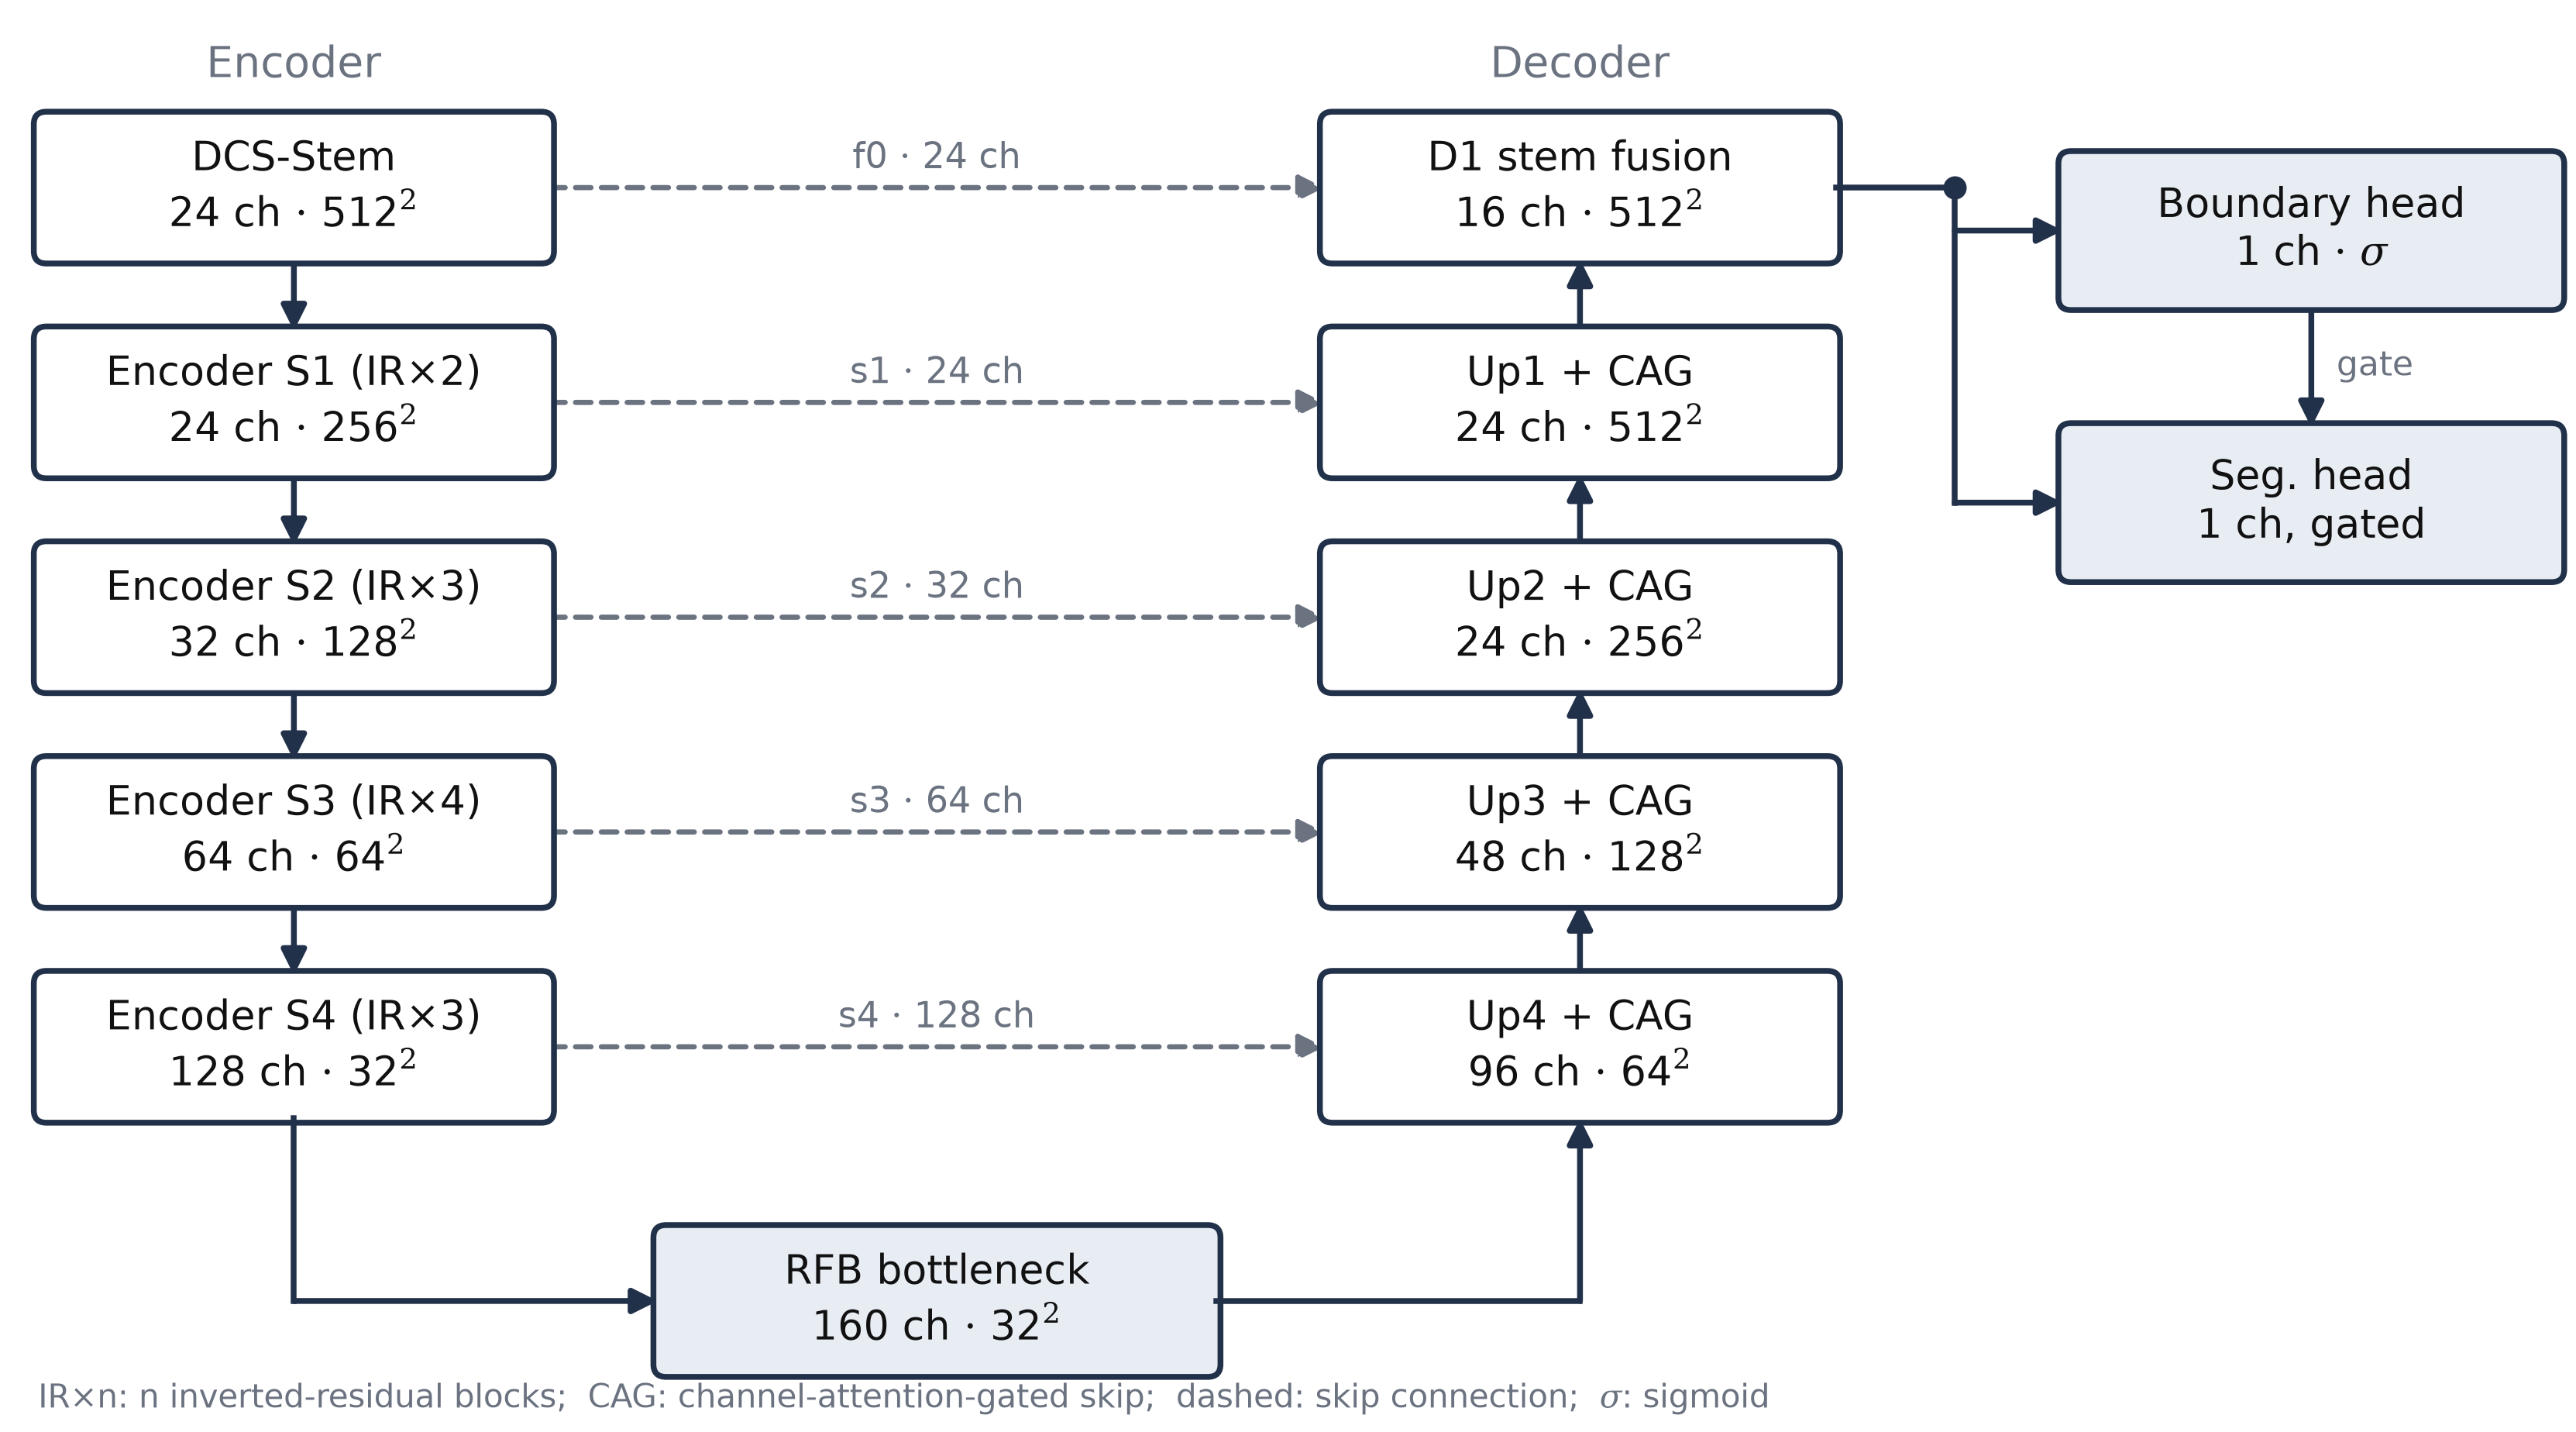
\includegraphics[width=0.93\textwidth]{figures/fig2_architecture.png}
\caption{MobileDFU-Net as implemented. DCS-Stem (24 ch at $512^2$); encoder stages S1--S4 with $2/3/4/3$ inverted-residual (IR) blocks at 24/32/64/128 channels and $256^2$/$128^2$/$64^2$/$32^2$; RFB bottleneck (160 ch at $32^2$); decoder Up4--Up1 (96/48/24/24 ch at $64^2$/$128^2$/$256^2$/$512^2$) with channel-attention-gated (CAG) skips; stem-fusion block $D_1$ (16 ch at $512^2$); auxiliary boundary head; and boundary-gated segmentation head. Dashed lines are skips. Input is raw RGB float32 in $[0,1]$ with no dataset-level normalization.}
\label{fig:architecture}
\end{figure*}

\subsection{Colour-Robust Stem}

The DCS-Stem (Fig.~\ref{fig:dcs}) splits the raw image into two paths. The structural path computes BT.601 luminance, a Sobel gradient magnitude, and a $3\times3$ convolution to 8 channels. The chromatic path applies ImageNet mean/std normalization only inside the network and a depthwise-separable convolution to 16 channels. A sigmoid gate $g$ derived from the structural features modulates the colour features, and the stem output is
\begin{equation}
F_0=\big[F_s,\;F_c\odot g\big],\qquad g=\sigma\big(W_s F_s\big),
\label{eq:dcs}
\end{equation}
where $F_s$ has 8 channels, $F_c$ has 16, $\odot$ is elementwise multiplication, and $[\cdot,\cdot]$ is channel concatenation, giving 24 channels at $512^2$. This is a structure-conditioned feature gate, not query--key--value cross-attention.

\begin{figure}[!t]
\centering
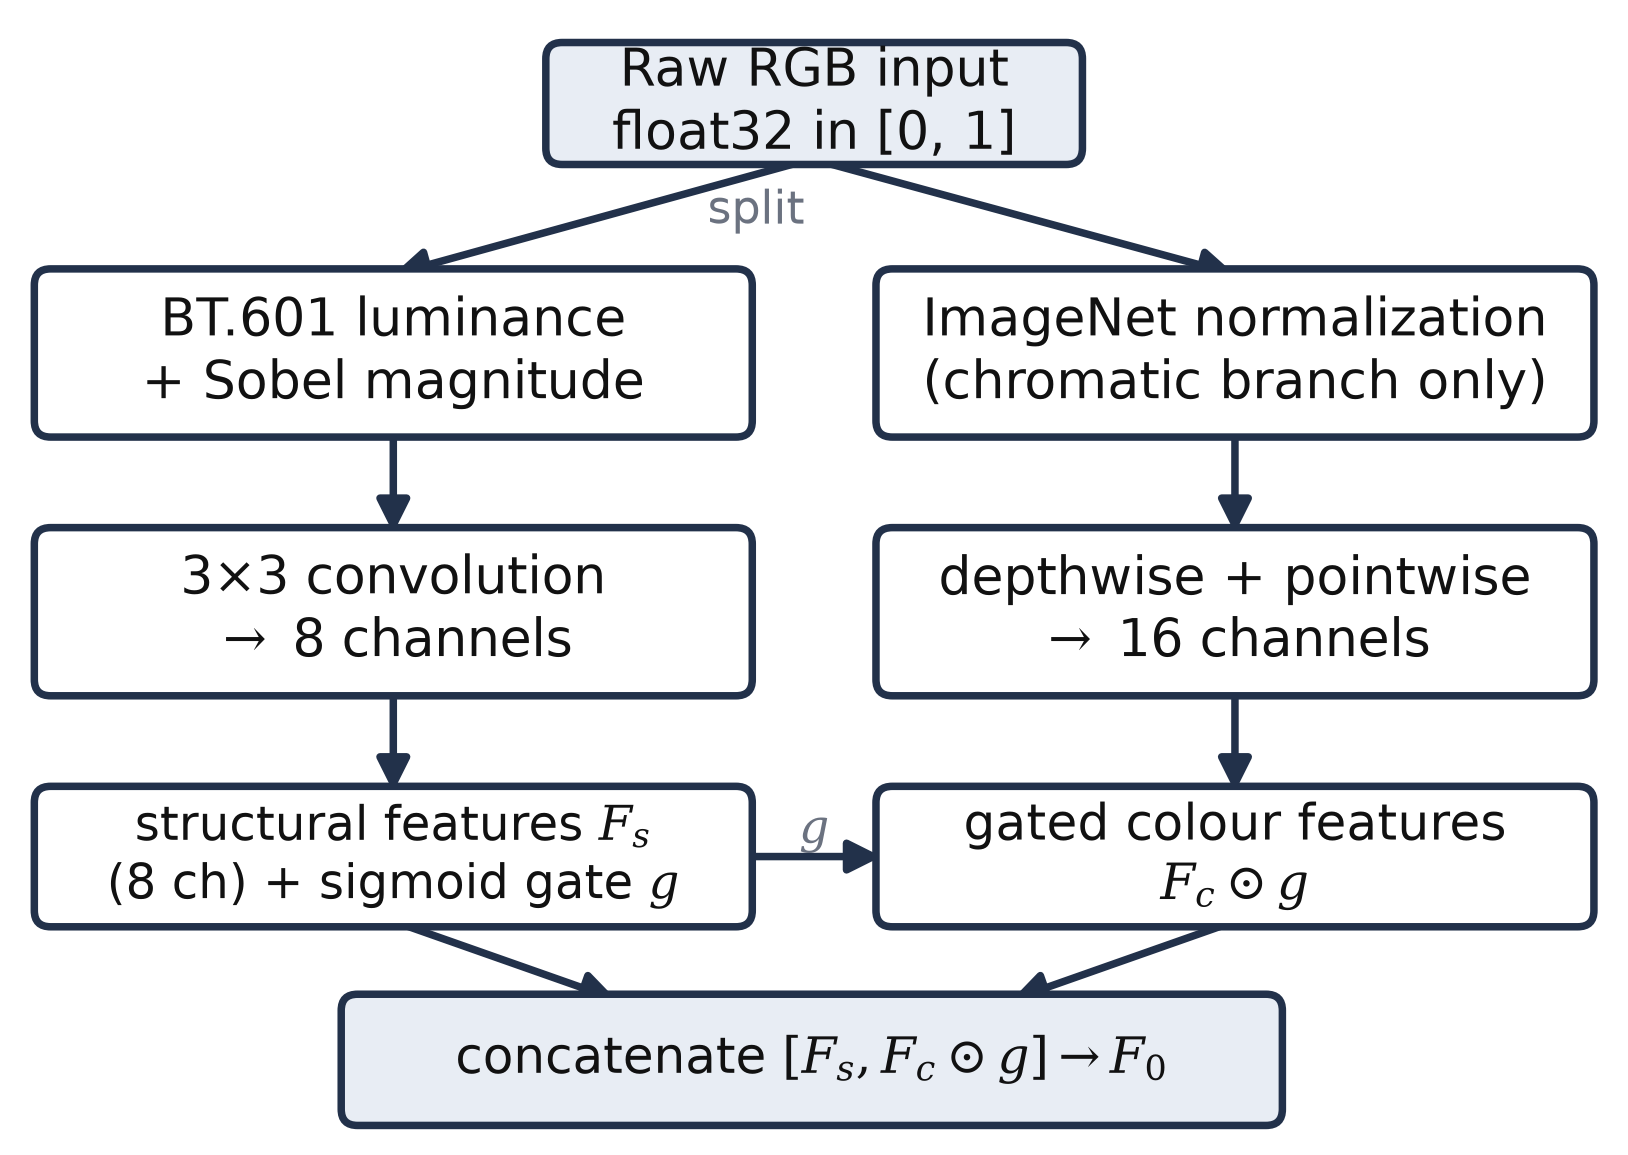
\includegraphics[width=0.94\columnwidth]{figures/fig3_dcs_stem.png}
\caption{DCS-Stem. Raw RGB is split into a luminance/Sobel structural path (8 channels) and an internally normalized chromatic path (16 channels). A sigmoid gate $g$ from the structural features modulates the colour features; the stem concatenates $F_s$ and $F_c\odot g$ into 24 channels.}
\label{fig:dcs}
\end{figure}

\subsection{Boundary-Aware Learning}

DFU boundaries are often faint and irregular, so an explicit boundary signal is used. The signed field is
\begin{equation}
\phi_{s}(x)=\phi_{fp}(x)-\phi_{fn}(x),
\label{eq:phisd}
\end{equation}
where $\phi_{fp}$ is positive in the exterior beyond the tolerance band and $\phi_{fn}$ is positive in the deep interior. The tolerance-aware linear boundary loss is
\begin{equation}
\mathcal{L}_{\mathrm{bd}}=\frac{1}{|\Omega|}\sum_{x\in\Omega}\phi_{s}(x)\,\sigma\big(z(x)\big),
\label{eq:bd}
\end{equation}
with segmentation logits $z$. Because the interior contribution is negative, $\mathcal{L}_{\mathrm{bd}}$ can be negative; it is not clamped. Fields are built by $3\times3$ erosion, a Euclidean distance transform, $\tau=2$, and a cap of 20 pixels, and are stored as float32 $[1,H,W]$. Empty masks produce zero fields and therefore zero boundary loss. Fig.~\ref{fig:boundary} summarizes the pipeline.

\begin{figure}[!t]
\centering
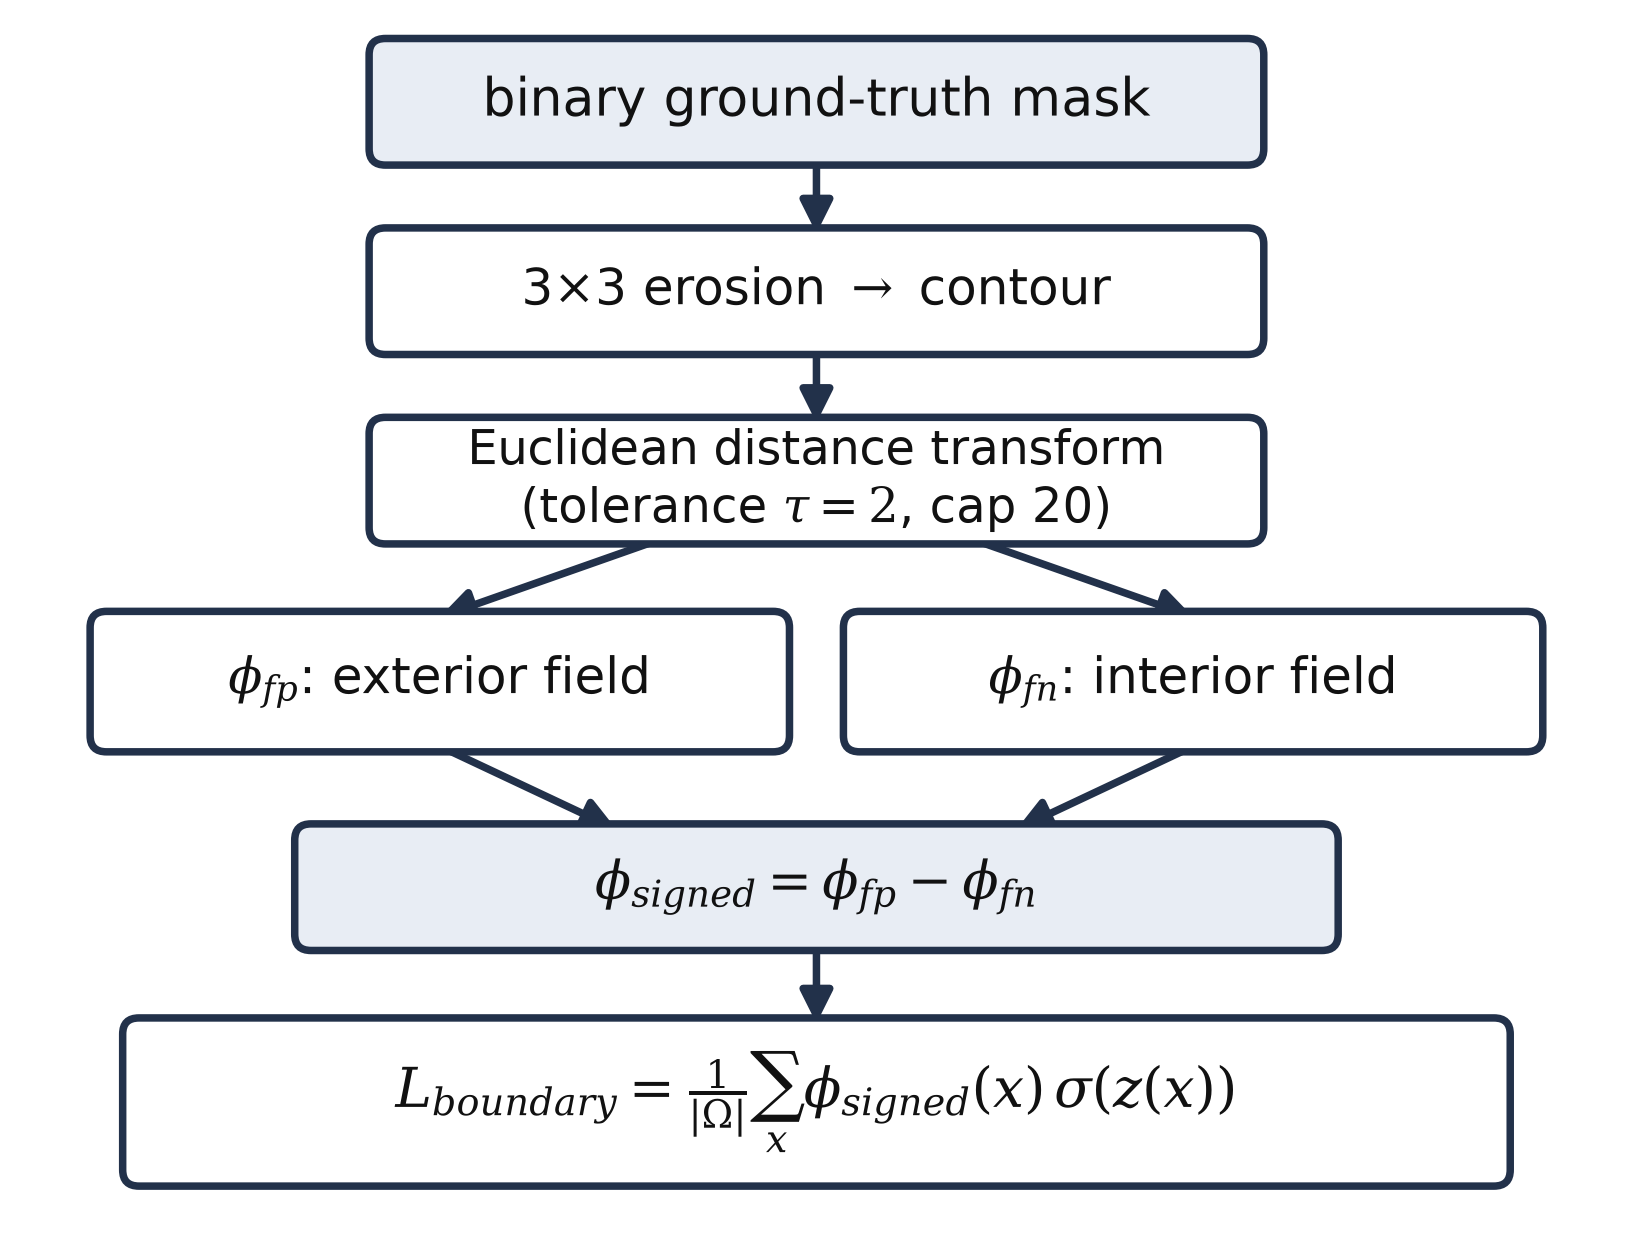
\includegraphics[width=0.92\columnwidth]{figures/fig4_boundary.png}
\caption{Boundary-field construction and loss. A mask is eroded to a contour, a Euclidean distance transform with tolerance $\tau=2$ and cap 20 yields exterior $\phi_{fp}$ and interior $\phi_{fn}$ fields, and the signed field weights the sigmoid segmentation probability.}
\label{fig:boundary}
\end{figure}

\subsection{Training Objective}

Let $p(x)=\sigma(z(x))$. The soft Dice loss is $1-\mathrm{Dice}$ computed on probabilities, with the empty-mask convention of the implementation. The positive-weighted binary cross-entropy is
\begin{equation}
\begin{aligned}
\mathcal{L}_{\mathrm{BCE}}=-\frac{1}{|\Omega|}\sum_{x\in\Omega}\Big[&w\,y(x)\log p(x)\\
&+\big(1-y(x)\big)\log\big(1-p(x)\big)\Big],
\end{aligned}
\label{eq:bce}
\end{equation}
with $w=2$ for the segmentation head and $w=2$ for the auxiliary boundary head in the baseline. The auxiliary head is trained with Dice plus BCE on a one-pixel morphological boundary. The total objective is
\begin{equation}
\mathcal{L}=\lambda_d\mathcal{L}_{\mathrm{Dice}}+\lambda_b\mathcal{L}_{\mathrm{BCE}}+\lambda_\phi\mathcal{L}_{\mathrm{bd}}+\lambda_a\mathcal{L}_{\mathrm{aux}},
\label{eq:total}
\end{equation}
with $(\lambda_d,\lambda_b,\lambda_\phi,\lambda_a)=(1.0,0.5,0.5,0.3)$.

\subsection{Uncertainty-Aware Inference}

At inference, dropout remains active in the four encoder dropout modules while BatchNorm stays in evaluation mode; module training flags are restored afterwards. Each of $T=15$ stochastic passes evaluates the original and horizontally flipped view in one batch, realigns the flipped logits, averages them, and applies the sigmoid. From the pass probabilities $p_t$,
\begin{equation}
\bar{p}(x)=\frac{1}{T}\sum_{t=1}^{T}p_t(x),\qquad
H[\bar{p}]=-\bar{p}\log\bar{p}-(1-\bar{p})\log(1-\bar{p}),
\label{eq:mc}
\end{equation}
and the mutual information is
\begin{equation}
I(x)=H[\bar{p}(x)]-\frac{1}{T}\sum_{t=1}^{T}H[p_t(x)].
\label{eq:mi}
\end{equation}
Tiny negative MI values in $[-10^{-7},0)$ are clamped to zero; larger negatives are retained. Entropy and MI are in nats. Fig.~\ref{fig:uncert} shows the pipeline. Predictive entropy is total uncertainty; MI is the epistemic component. Neither is a calibration metric.

\begin{figure}[!t]
\centering
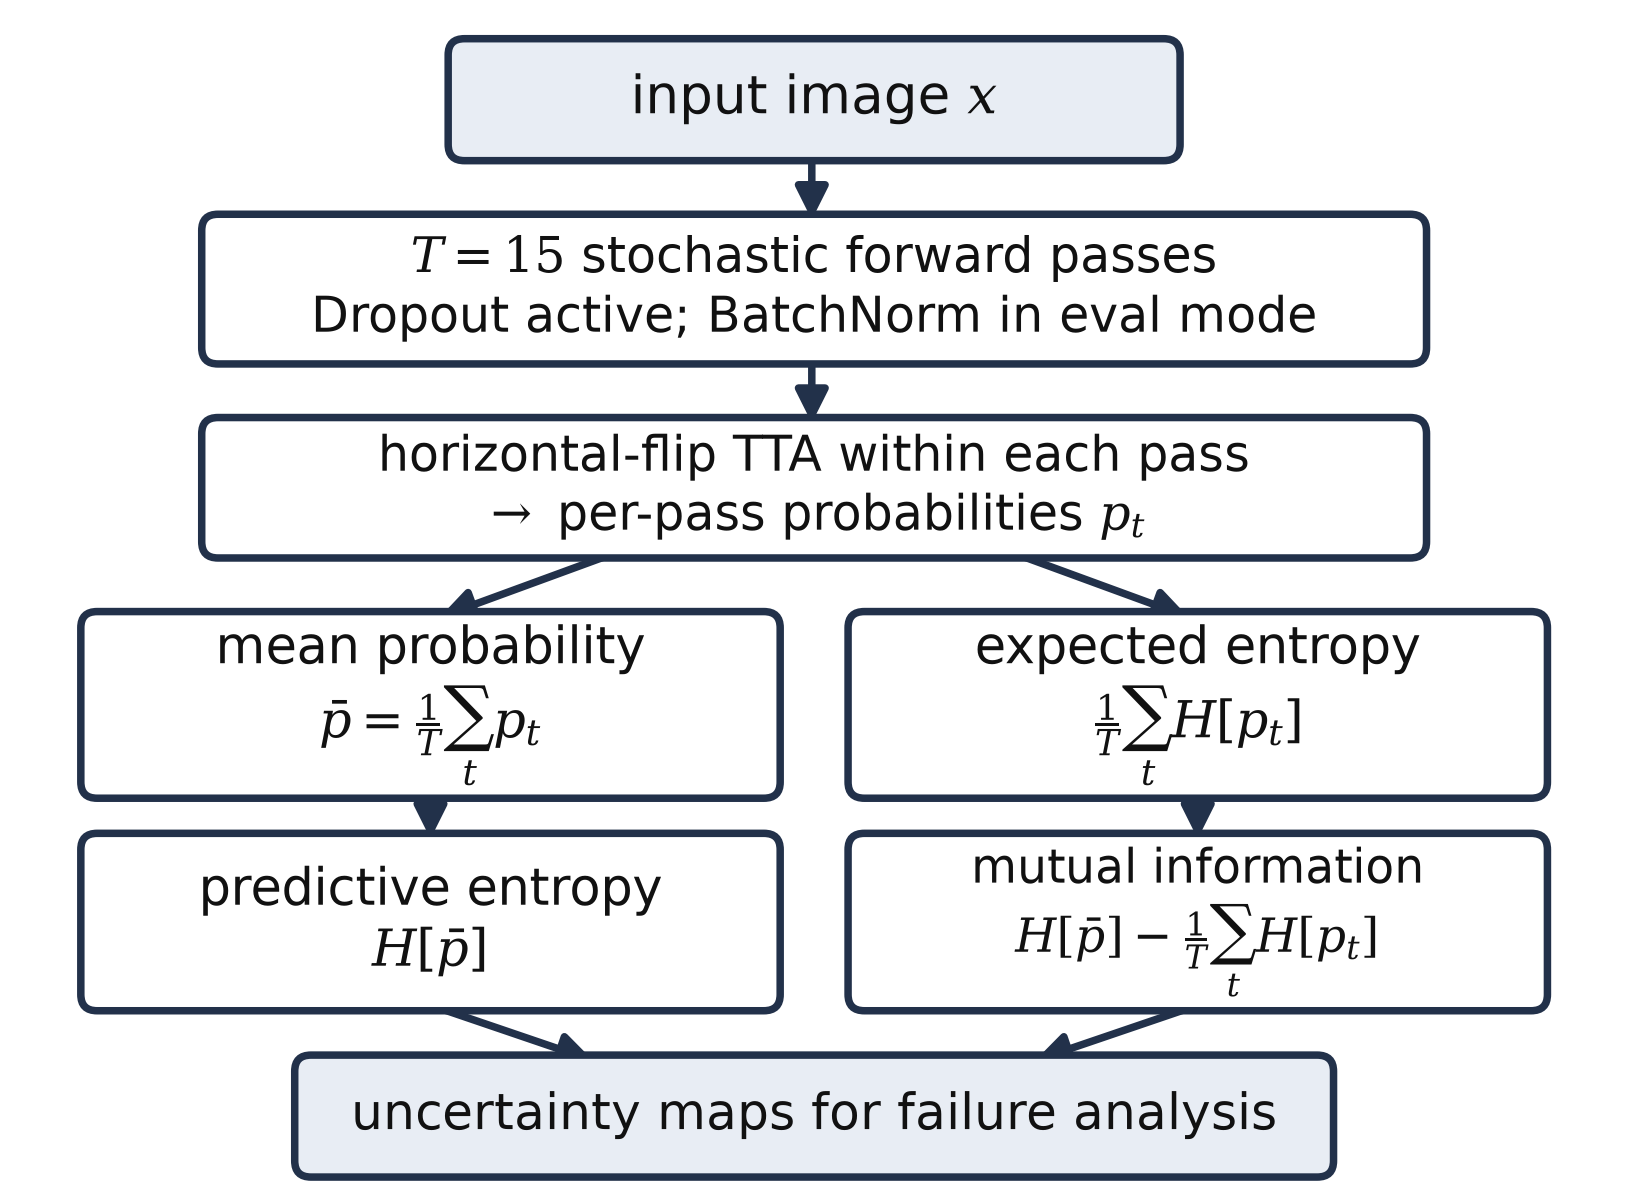
\includegraphics[width=0.92\columnwidth]{figures/fig5_uncertainty.png}
\caption{Uncertainty inference: $T=15$ stochastic passes with dropout active and BatchNorm in evaluation mode, horizontal-flip TTA per pass, mean probability, predictive entropy, and mutual information.}
\label{fig:uncert}
\end{figure}

\subsection{Training Protocol}

Three runs used seeds 42, 1337, and 2024 with the same approved cohort and preprocessing. Table~\ref{tab:training} lists the configuration, with values marked as recorded for Seed 2024 where the other runs were not re-verified from their own notebooks. Seed 42 and Seed 2024 completed 100 epochs; Seed 1337 resumed from epoch 21 and was stopped by early stopping after epoch 96. The native target was never used for training, model selection, or threshold tuning.

\begin{table}[!t]
\centering
\caption{Training configuration (values marked $^\ast$ recorded for Seed 2024)}
\label{tab:training}
\begin{tabular}{@{}ll@{}}
\toprule
Parameter & Value \\
\midrule
Seeds & 42, 1337, 2024 \\
Configured epochs & 100 per seed \\
Batch size & 8 \\
Input resolution & $512\times512$ \\
Precision & FP32 (AMP disabled) \\
Optimizer$^\ast$ & AdamW ($\beta_1=0.9$, $\beta_2=0.999$) \\
Learning rate$^\ast$ & $5\times10^{-4}$ \\
Weight decay$^\ast$ & $1\times10^{-4}$ \\
Early-stopping patience$^\ast$ & 15 epochs \\
Loss weights & 1.0 / 0.5 / 0.5 / 0.3 \\
BCE positive weight & 2.0 (segmentation and auxiliary) \\
Boundary $\tau$ / cap & 2 / 20 pixels \\
Training / validation records & 927 / 186 \\
Native target in training & No \\
GPU & Tesla T4 (Kaggle) \\
\bottomrule
\end{tabular}
\end{table}

\subsection{Evaluation Protocol and Profiling}

The primary reported metric is macro Dice at threshold $\tau=0.5$. Cross-dataset values were produced once on the frozen native target for each best checkpoint. We also report IoU, sensitivity, specificity, and micro Dice. Internal-validation IoU, sensitivity, specificity, and boundary-quality metrics were not logged for all seeds and are not reconstructed here; only the MC Dropout diagnostic reports them for Seed 2024. Computational cost was measured on an NVIDIA RTX 2050 (4~GB, PyTorch 2.11.0, CUDA 12.8) with batch size 1, $512\times512$ FP32 input, model in evaluation mode, no gradients, five warm-up and twenty timed iterations. We use fvcore for convolution/linear FLOPs and report both conventions:
\begin{equation}
\mathrm{GFLOPs}=2\times\mathrm{GMACs},
\label{eq:flops}
\end{equation}
because one multiply--accumulate is two floating-point operations. fvcore counts only convolution and linear operators, so its value is a lower bound; torch.profiler additionally counts some elementwise operators.

\section{Results}
\label{sec:results}

\subsection{Internal Validation Across Seeds}

Table~\ref{tab:seeds} and Fig.~\ref{fig:performance}(a) report the best internal-validation Dice. The mean was $0.8339\pm0.0027$ (sample standard deviation). This dispersion is small but describes three seeds on one source cohort; it is not evidence of cross-dataset robustness.

\begin{table}[!t]
\centering
\caption{Best internal-validation Dice per seed}
\label{tab:seeds}
\begin{tabular}{@{}lcccc@{}}
\toprule
Seed & Best Dice & Epoch & Epochs run & Outcome \\
\midrule
42   & 0.8370 & 99 & 100 & completed \\
1337 & 0.8322 & 81 & 96  & early stop \\
2024 & 0.8326 & 87 & 100 & completed \\
\bottomrule
\end{tabular}
\end{table}

Epoch numbers follow the convention that the stored \texttt{best\_epoch} is zero-based and the human-readable epoch is the stored value plus one: stored 98, 80, and 86 become 99, 81, and 87.

\subsection{Training Behaviour}

Fig.~\ref{fig:training} shows the Seed 2024 history. Training and validation loss fell quickly and then plateaued, while validation Dice rose to 0.8326 at epoch 87 and ended at 0.8267 at epoch 100. The best checkpoint therefore did not coincide with the last epoch. Seed 42 peaked at 0.8370 at epoch 99, essentially at the end of training, with final training loss 0.2275 and validation loss 0.3333. Seed 1337 peaked at 0.8322 at epoch 81 and stopped after epoch 96. No run was selected using target data.

\begin{figure}[!t]
\centering
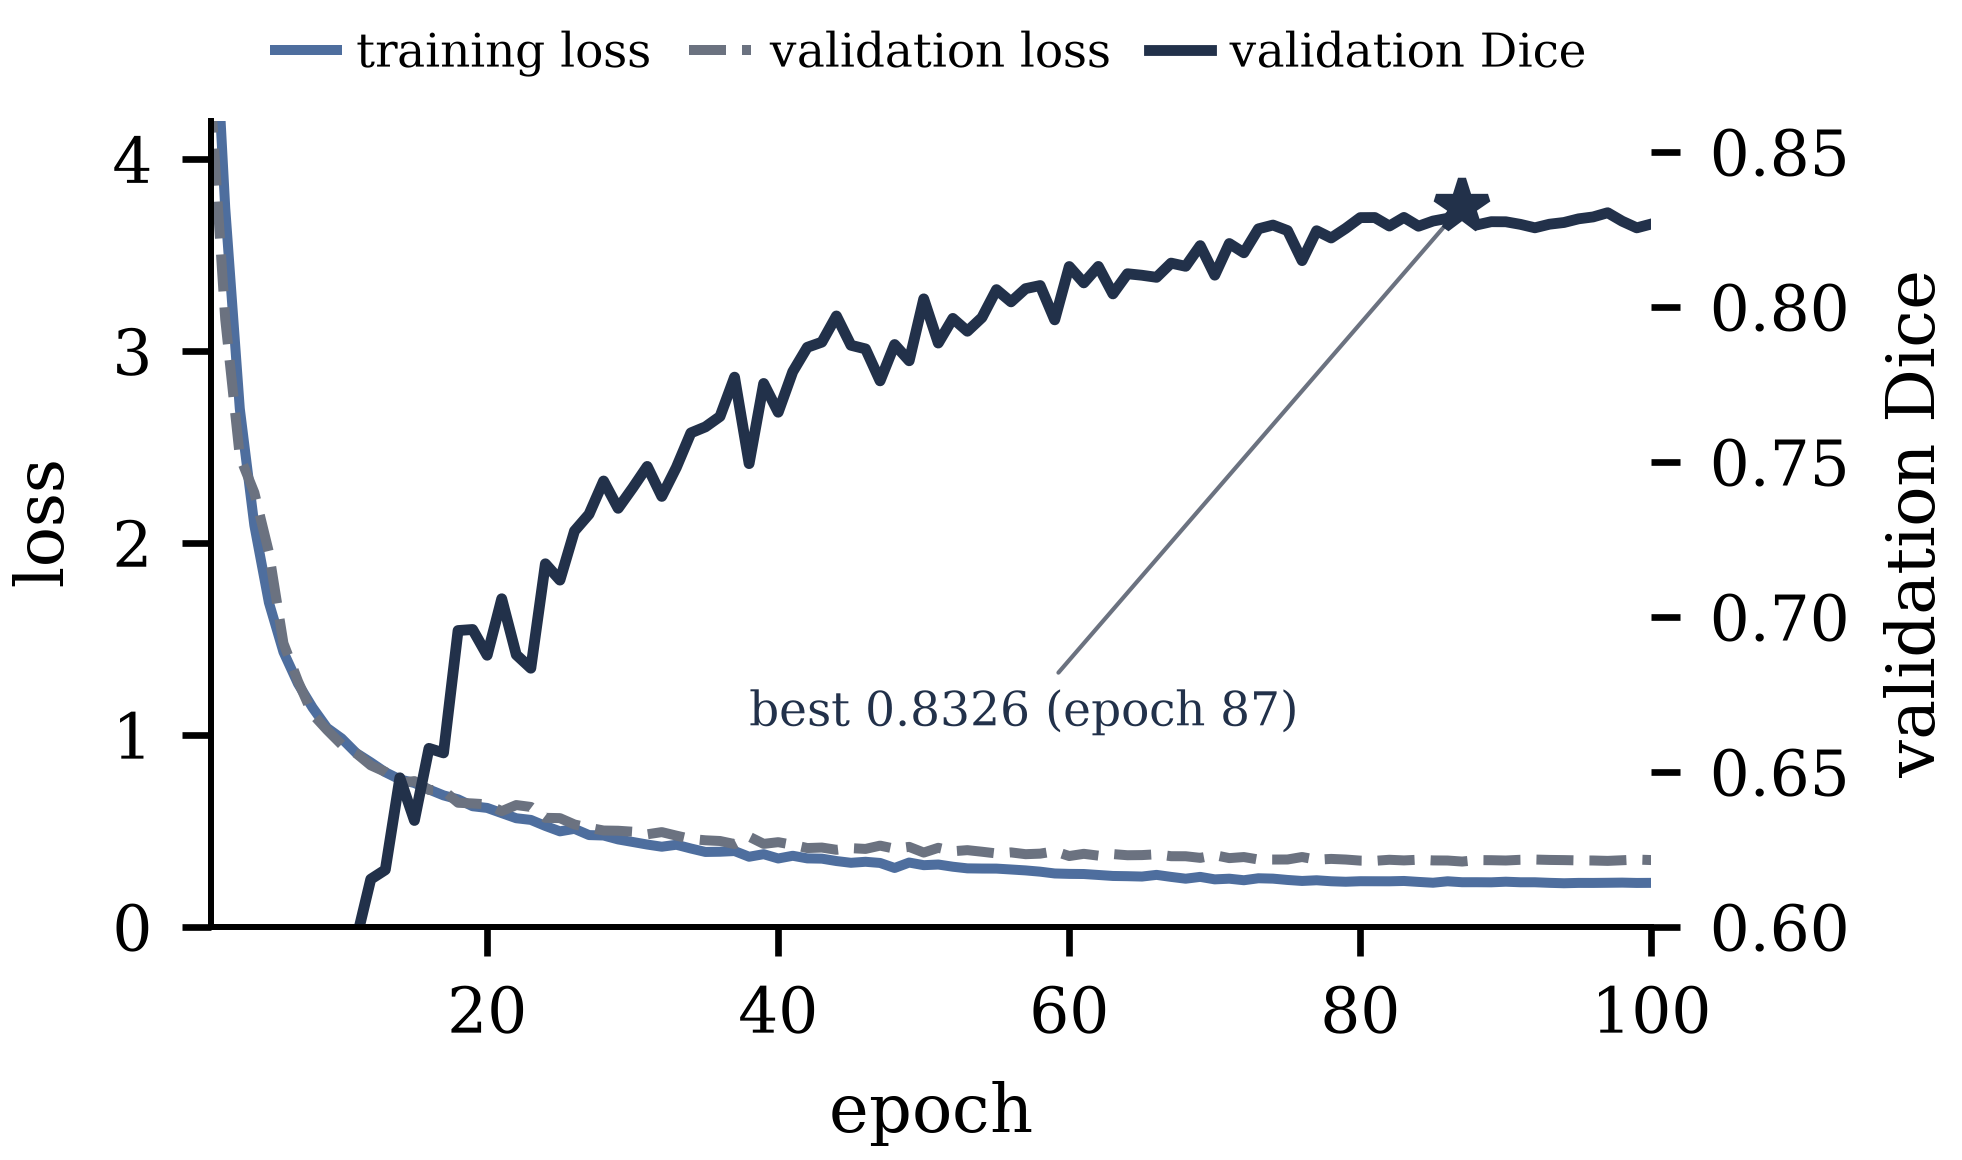
\includegraphics[width=0.95\columnwidth]{figures/fig7_training.png}
\caption{Seed 2024 training history: training and validation loss (left axis) and validation Dice (right axis). The star marks the best checkpoint at human-readable epoch 87 (stored \texttt{best\_epoch}=86).}
\label{fig:training}
\end{figure}

\subsection{Model Complexity}

The model has 1,116,883 parameters and a 4.47~MB FP32 checkpoint. fvcore reports 4.209~GFLOPs and 2.1045~GMACs for convolution and linear operators; ptflops reports 4.18~GMACs, consistent with the same MAC convention, and torch.profiler reports 7.8217~GFLOPs when convolution, multiplication, and addition are partially counted. The fvcore value is a lower bound because hardswish, sigmoid, sqrt, and dropout are not counted. Mean latency was 75.55~ms (median 75.26, min 74.84, max 77.82), throughput 13.24 images/s, and peak GPU memory 245~MB allocated and 316~MB reserved. These measurements used synthetic input on an RTX 2050, not the Kaggle T4 used for training, and should not be read as a clinical deployment benchmark.

\subsection{Cross-Dataset Evaluation}

Table~\ref{tab:native} and Fig.~\ref{fig:performance}(b)--(c) show the frozen native-target results at $\tau=0.5$. Macro Dice fell from 0.83 internally to 0.22--0.25, a gap of roughly 0.59--0.62 Dice. Sensitivity was only 0.17--0.21, whereas specificity stayed above 0.99: the model predicted too little foreground, not too much. Seed 42 was best on the target, but the spread across seeds (0.2203--0.2485) is an order of magnitude smaller than the gap to internal performance.

\begin{table}[!t]
\centering
\caption{Cross-dataset evaluation on the frozen native target cohort ($n=2{,}187$, threshold 0.5)}
\label{tab:native}
\scriptsize
\setlength{\tabcolsep}{3.6pt}
\begin{tabular}{@{}lccccc@{}}
\toprule
Seed & Dice & IoU & Sens. & Spec. & Micro Dice \\
\midrule
42   & 0.2485 & 0.1658 & 0.2098 & 0.9914 & 0.2457 \\
2024 & 0.2365 & 0.1566 & 0.1933 & 0.9915 & 0.2420 \\
1337 & 0.2203 & 0.1469 & 0.1742 & 0.9951 & 0.2230 \\
\bottomrule
\end{tabular}
\end{table}

\begin{figure*}[!tb]
\centering
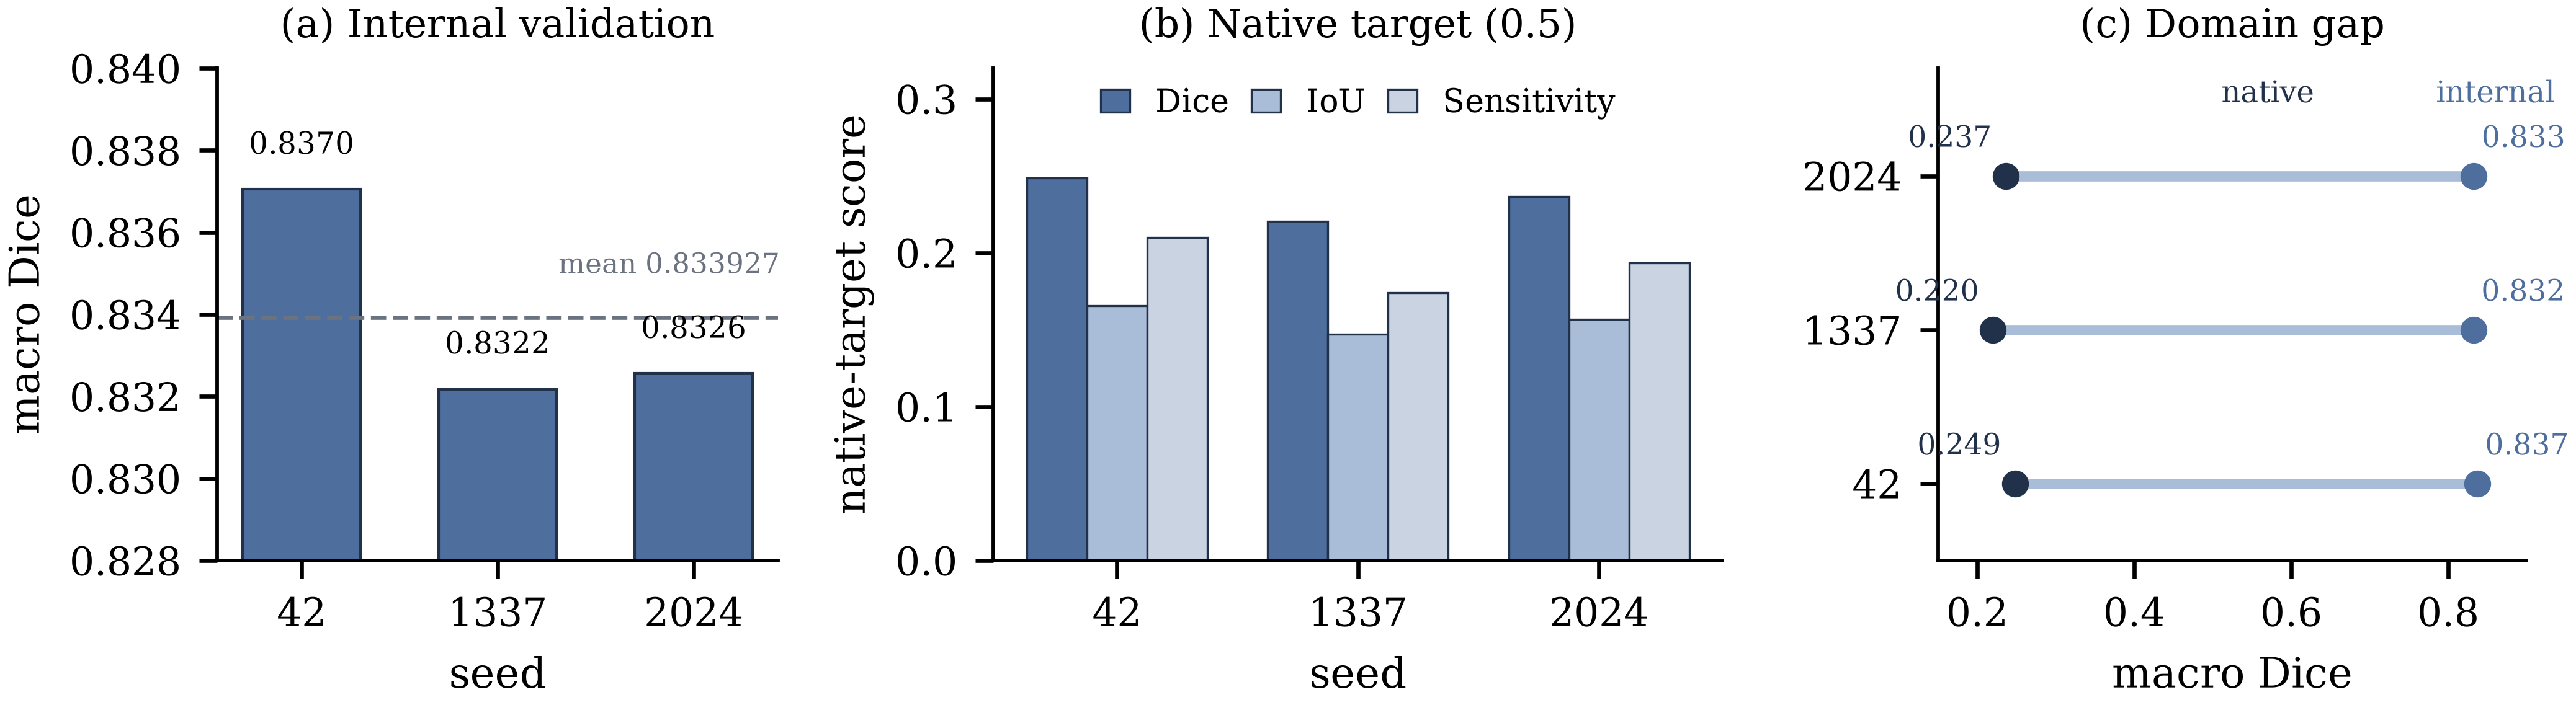
\includegraphics[width=\textwidth]{figures/fig6_performance.png}
\caption{Three-seed performance. (a) Best internal-validation macro Dice; the dashed line is the three-seed mean 0.833927. (b) Native-target Dice, IoU, and sensitivity at threshold 0.5. (c) Interval from native-target Dice (left dot) to internal Dice (right dot) for each seed, showing a gap of about 0.59--0.62.}
\label{fig:performance}
\end{figure*}

\subsection{Wound-Size Stratification}

Using the Seed 2024 MC Dropout per-image outputs, we stratified the 2,187 target images by ground-truth wound area into quartiles (Q1 $\leq$ 8,995; Q2 $\leq$ 22,237; Q3 $\leq$ 42,706; Q4 $\leq$ 185,768 pixels; $n=547,547,546,547$). Median Dice fell monotonically from 0.1873 in Q1 to 0.0764 in Q4, median sensitivity fell from 0.1325 to 0.0401, median false-negative fraction rose from 0.8675 to 0.9599, and median predicted-to-reference area ratio fell from 0.3006 to 0.0521. These are descriptive associations on one seed and one target cohort; they do not establish that wound size causes failure, although they are consistent with the model retreating to small or empty predictions as lesions grow.

\subsection{Uncertainty and Failure Detection}

Table~\ref{tab:uncert} reports MC Dropout results for the Seed 2024 checkpoint (best epoch 87, $T=15$). On internal validation, MC inference gave 0.8347 Dice with very low mean entropy (0.00191) and MI (0.00055). On the native target, Dice was 0.2135, mean entropy 0.01789, and mean MI 0.00791. Entropy and MI correlated only weakly with Dice (Spearman $\rho=0.370$ and $0.344$).

For failure defined as Dice $<$ 0.1 (966 images, 44.17\%), the AUROC was 0.300 for entropy and 0.311 for MI. Because values below 0.5 indicate anti-correlation, failures had \emph{lower} mean entropy (0.0111) than successes (0.0233), and lower mean MI (0.00505 versus 0.01018). In other words, the model was often confidently wrong. These AUROCs are exploratory image-level statistics and do not establish calibration or clinical utility.

\begin{table}[!t]
\centering
\caption{Uncertainty evaluation on the internal-validation ($n=186$) and native-target ($n=2{,}187$) cohorts. Deterministic rows use one pass; MC rows use the Seed 2024 checkpoint with $T=15$. Entropy and MI are in nats.}
\label{tab:uncert}
\scriptsize
\setlength{\tabcolsep}{2.6pt}
\begin{tabular}{@{}lccccc@{}}
\toprule
& & & & \multicolumn{2}{c}{Failure AUROC} \\
\cmidrule(lr){5-6}
Cohort / protocol & Dice & Ent. & MI & Ent. & MI \\
\midrule
Internal, det. & 0.8326 & N/A & N/A & N/A & N/A \\
Internal, MC  & 0.8347 & 0.00191 & 0.00055 & NE & NE \\
Native, det. & 0.2365 & N/A & N/A & N/A & N/A \\
Native, MC  & 0.2135 & 0.01789 & 0.00791 & 0.300 & 0.311 \\
\bottomrule
\end{tabular}

\vspace{2pt}
{\scriptsize N/A: not applicable---a deterministic single pass produces no MC entropy, MI, or failure AUROC. NE: not evaluated---no internal failure-label set was defined for AUROC. AUROC is for Dice $<$ 0.1 failure; values below 0.5 indicate anti-correlation.}
\end{table}

\subsection{Foreground-Recovery Intervention}

A fresh Seed 2024 run raised the segmentation BCE positive weight from 2 to 4 while keeping the auxiliary weight at 2. Table~\ref{tab:recovery} and Fig.~\ref{fig:recovery} show the result. Internal Dice fell slightly to 0.8225. Native Dice rose by 0.0071 to 0.2436 and sensitivity by 0.0177 to 0.2110. The predefined targets were $+0.02$ Dice and $+0.05$ sensitivity; both failed. Only the guardrail of internal Dice $\geq0.82$ passed. A threshold sweep selected 0.75 on internal validation (Dice 0.8240); on the target, Dice at 0.75 was 0.2328, lower than 0.2436 at 0.5 and 0.2547 at 0.25. The target threshold curve was descriptive only and did not influence selection.

\begin{table}[!t]
\centering
\caption{Foreground-recovery experiment (positive weight 2 $\rightarrow$ 4)}
\label{tab:recovery}
\begin{tabular}{@{}lccc@{}}
\toprule
Metric & Baseline & New & Delta \\
\midrule
Internal macro Dice & 0.8326 & 0.8225 & $-0.0101$ \\
Native macro Dice & 0.2365 & 0.2436 & $+0.0071$ \\
Native sensitivity & 0.1933 & 0.2110 & $+0.0177$ \\
Native macro IoU & 0.1566 & 0.1632 & $+0.0066$ \\
\bottomrule
\end{tabular}
\end{table}

\begin{figure}[!t]
\centering
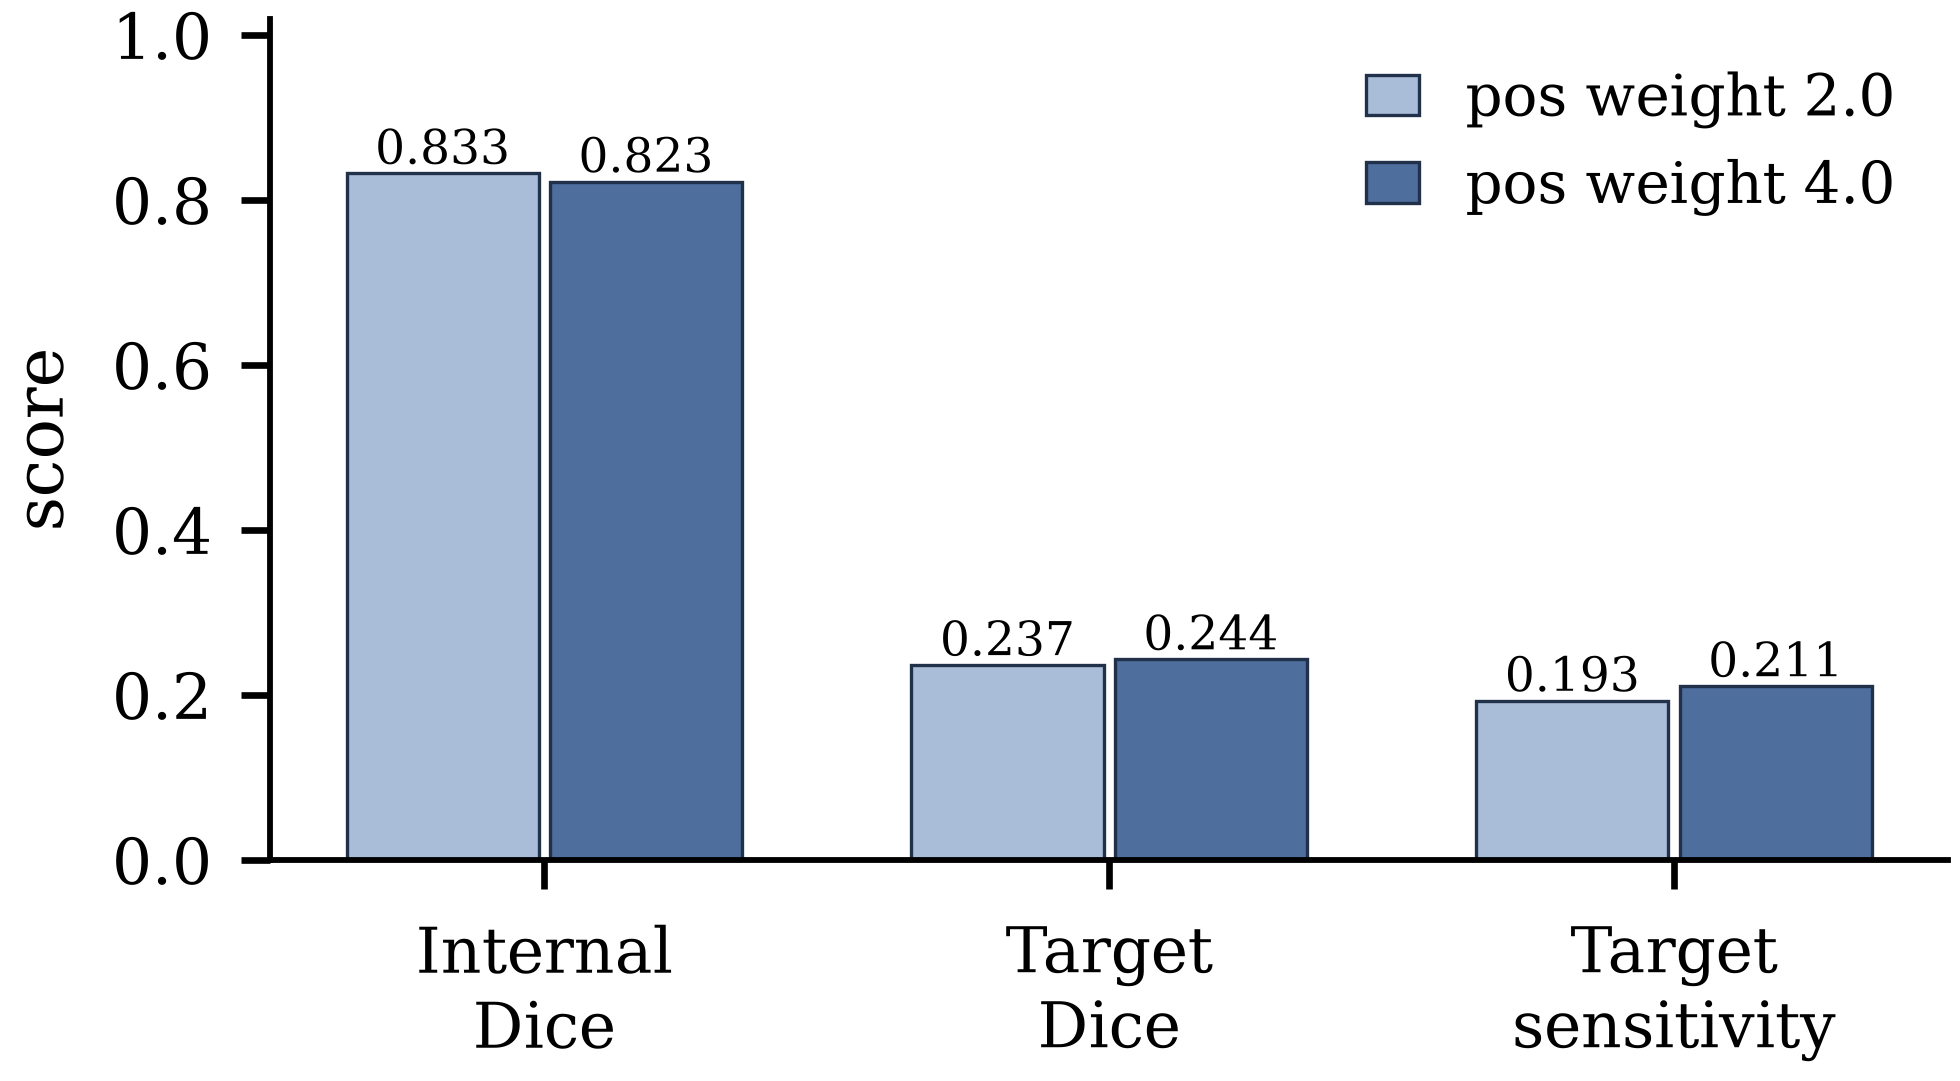
\includegraphics[width=0.92\columnwidth]{figures/fig9_recovery.png}
\caption{Foreground-recovery intervention on Seed 2024. Raising the segmentation positive weight from 2 to 4 reduced internal Dice and produced only small gains on native-target Dice and sensitivity, below the predefined targets.}
\label{fig:recovery}
\end{figure}

\subsection{Colour and Boundary Ablations}

Two Seed 42 ablations were evaluated on the frozen target (Table~\ref{tab:ablation}, Fig.~\ref{fig:ablation}). E1 removed the DCS-Stem (the colour ablation); E2 zeroed the boundary logits and probabilities. Both degraded every reported native metric. E1 reduced Dice to 0.2398 and sensitivity to 0.1873. E2 was worse, with Dice 0.2067 and sensitivity 0.1649, indicating that the boundary supervision contributed materially.

Paired per-image analysis over 2,187 matched records gave a mean $\Delta$Dice of $-0.00869$ for E1 (957 improved, 1,081 deteriorated, 149 unchanged) and $-0.04180$ for E2 (684 improved, 1,303 deteriorated, 200 unchanged). By wound-area quartile, E1 was positive only in Q1 ($+0.00535$) and negative elsewhere; E2 was negative in all quartiles and worst in Q3.

E2 also removes meaningful boundary supervision rather than only disabling one loss term: with \texttt{boundary\_ablation=True}, boundary logits and probabilities are forced to zero, the boundary loss becomes 0.0, and boundary-head parameters receive gradients of order $7\times10^{-5}$. Restoring both components recovers the baseline, so this is not a novel combined intervention.

\begin{table}[!t]
\centering
\caption{Native-target ablation results (Seed 42, $n=2{,}187$, threshold 0.5)}
\label{tab:ablation}
\footnotesize
\begin{tabular}{@{}lccc@{}}
\toprule
Metric & Baseline & E1 colour & E2 boundary \\
\midrule
Macro Dice & 0.2485 & 0.2398 & 0.2067 \\
Macro IoU & 0.1658 & 0.1590 & 0.1355 \\
Macro sensitivity & 0.2098 & 0.1873 & 0.1649 \\
Macro specificity & 0.9914 & 0.9933 & 0.9935 \\
Micro Dice & 0.2457 & 0.2287 & 0.2025 \\
\bottomrule
\end{tabular}
\end{table}

\begin{figure*}[!tb]
\centering
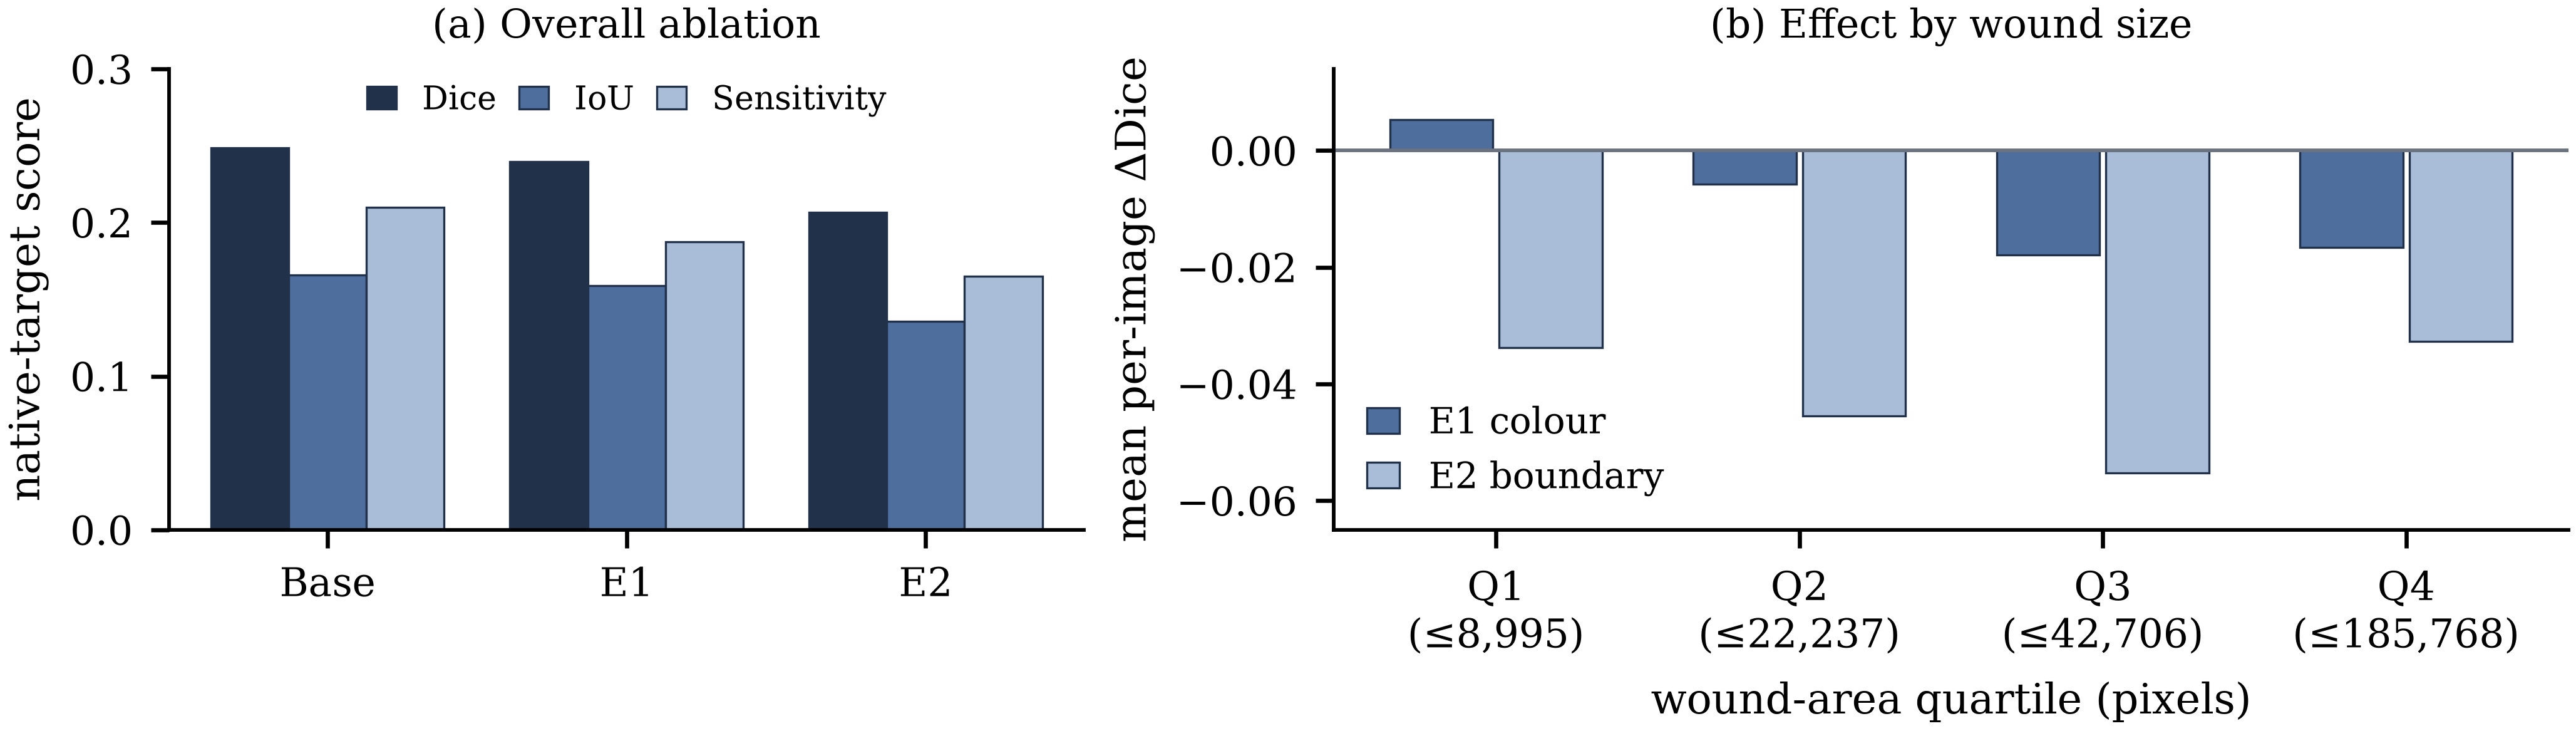
\includegraphics[width=\textwidth]{figures/fig8_ablation.png}
\caption{Ablations on the native target (Seed 42). (a) Baseline versus E1 (no DCS-Stem) and E2 (boundary logits/probabilities zeroed). (b) Mean per-image $\Delta$Dice by ground-truth wound-area quartile; E1 is positive only in the smallest-wound quartile, and E2 is negative everywhere.}
\label{fig:ablation}
\end{figure*}

\subsection{Artifact Integrity}

Independent artifact verification was completed for Seed 2024. Notebook source, training log, \texttt{best.pt}, \texttt{last.pt}, RNG-state file, and kernel log were compared across primary and backup copies and matched. The external log contained 87 records for epochs 13--99; \texttt{last.pt} contained 100 embedded history records for epochs 0--99. All 87 overlapping validation Dice values matched within $10^{-12}$, with zero mismatches. A structural comparison between the local model and the recovered checkpoints found 517 tensors, zero missing keys, zero unexpected keys, and zero shape mismatches. This establishes structural compatibility, not a completed strict \texttt{load\_state\_dict()} execution. Equivalent verification has not yet been performed for Seeds 42 and 1337.

\section{Discussion}
\label{sec:discussion}

The central empirical fact is the size of the domain gap: about 0.59--0.62 macro Dice between internal validation and the native target, with sensitivity below 0.22. Because specificity remained above 0.99, the failure is not diffuse noise but a systematic retreat from foreground. The wound-size gradient is consistent with a model that becomes more conservative as the lesion grows, although the present design cannot identify the causal mechanism.

The ablations are informative precisely because both are negative. Removing the DCS-Stem lowered native Dice by 0.0087 on average and by more in larger-wound quartiles, so the colour/structure split helps, but only marginally relative to the total gap. Removing the boundary signal lowered Dice by 0.0418, which is a larger effect than the colour stem and suggests that boundary supervision is the more consequential of the two components. Neither component closes the gap, and the baseline itself remains far from usable cross-dataset accuracy.

The recovery experiment shows that class weighting alone is not enough. A positive weight of 4 moved native Dice by 0.007 and sensitivity by 0.018, at the cost of internal Dice. This is a weak trade and is consistent with the view that the failure is representational and domain-related, not simply a decision-threshold or class-imbalance problem.

The uncertainty results are the most cautionary. AUROC below 0.5 means that entropy and MI ranked failures worse than chance, and the mean values show the direction: failed images had lower entropy than successful ones. A clinician-facing system that used these maps as a deferral signal would defer the wrong cases. The result does not show that uncertainty estimation is useless in general; it shows that this MC Dropout configuration, trained on this source cohort, does not provide a reliable failure score on this target.

The study also has a structural limitation that no modelling choice can remove: two lineage groups are not a multi-centre validation. The source and target differ in acquisition and colour, but they do not sample the space of clinical sites, cameras, skin tones, or ulcer etiologies. The reported target numbers should therefore be read as a single stress test, not as an estimate of expected clinical performance.

\section{Limitations}
\label{sec:limitations}

\begin{enumerate}
\item \textbf{Dataset lineage and generalizability.} Only two independent lineage groups were available (AZH, sharing lineage with FUSeg; WSEG/Mendeley, sharing lineage with each other); DFUC 2022 was unused, so this is not broad, multi-centre external validation. A label-uncertainty review found lesion-like features in 22 of 25 sampled empty-mask records, motivating exclusions without fully characterising residual label noise. The three-seed results are internal-validation results on one source cohort, not cross-dataset results, and their dispersion is not domain robustness.
\item \textbf{Training reproducibility and checkpoint verification.} Seed 1337 stopped early at epoch 96 and full per-epoch logs were unavailable for Seeds 42 and 1337; only Seed 2024 received full artifact verification. Strict \texttt{load\_state\_dict()} loading and local inference reproduction remain pending, and the Seed 2024 structural comparison is not a substitute.
\item \textbf{Uncertainty calibration and intervention scope.} ECE and Brier calibration metrics were not computed, so uncertainty is characterised only by entropy, MI, rank correlation and AUROC. The foreground-recovery experiment tested one intervention (positive weight 2 to 4) at one value, with no combined intervention; both ablations and recovery were negative on the target, and E2 removed boundary supervision substantially.
\item \textbf{Computational profiling and clinical validation.} Profiling used synthetic input on an RTX 2050 rather than the training GPU, and FLOP counts are lower bounds. No clinical, prospective or regulatory validation was performed, and no clinical-readiness claim is made.
\end{enumerate}

\section{Future Work}
\label{sec:future}

The following items are genuinely pending and are not restatements of completed work:
\begin{enumerate}
\item Execute strict \texttt{load\_state\_dict()} loading and reproduce the recorded best internal-validation scores for all three seeds.
\item Recover and verify complete per-epoch training and validation logs for Seeds 42 and 1337, analogous to the Seed 2024 verification.
\item Compute per-pixel calibration and reliability metrics (ECE, Brier score, reliability diagrams) once the required per-pixel outputs are available.
\item Evaluate combined foreground-recovery interventions, such as recall-oriented loss, stronger colour and illumination augmentation, and boundary emphasis, rather than positive weighting alone.
\item Extend evaluation to additional independent lineage groups, subject to data-access and licence constraints, and report each group separately.
\item Study target-side adaptation methods under a protocol that keeps the target labels strictly held out, so that adaptation and evaluation are not conflated.
\end{enumerate}

\section{Conclusion}
\label{sec:conclusion}

This paper reported MobileDFU-Net, a lightweight DFU segmentation framework with a decoupled chromatic--structural stem, a tolerance-aware signed-distance boundary loss, and MC Dropout uncertainty inference. An audited reconciliation established 927 source-training and 186 internal-validation records and a 2,187-record native target, while documenting that only two independent lineage groups were available. Three seeds reached internal-validation Dice of 0.8370, 0.8322, and 0.8326, but the same checkpoints reached only 0.2485, 0.2365, and 0.2203 macro Dice on the target, with sensitivity below 0.22. A positive-weight intervention gave a small, insufficient gain; colour and boundary ablations both degraded target performance; and entropy/MI failure detection was anti-correlated with failure (AUROC 0.300/0.311). We conclude that the domain gap, foreground suppression, and uncertainty reliability remain open problems for this framework, and we have reported the negative results rather than presenting a partial success as a solution.

\section*{Acknowledgment}

The authors thank the providers of the AZH and WSEG/Mendeley wound-image datasets whose data and documentation made this investigation possible, and the developers of the open-source PyTorch, fvcore, and ptflops tools used for implementation and profiling. No funding, institutional endorsement, or dataset permission beyond those already described in the text is claimed.

\bibliographystyle{IEEEtran}
\bibliography{references}

\end{document}
